% !TeX root = RJwrapper.tex
\title{Will the Real Hopkins Statistic Please Stand Up?}
\author{by Kevin Wright}

\maketitle

\abstract{%
Hopkins statistic (Hopkins and Skellam 1954) can be used to test for spatial randomness of data and for detecting clusters in data. Although the method is nearly 70 years old, there is persistent confusion regarding the definition and calculation of the statistic. We investigate the confusion and its possible origin. Using the most general definition of Hopkins statistic, we perform a small simulation to verify its distributional properties, provide a visualization of how the statistic is calculated, and provide a fast R function to correctly calculate the statistic. Finally, we propose a protocol of five questions to guide the use of Hopkins statistic.
}

\hypertarget{introduction}{%
\section{Introduction}\label{introduction}}

Hopkins and Skellam (1954) introduced a statistic to test for spatial randomness of data. If the null hypothesis of spatial randomness is rejected, then one possible interpretation is that the data may be clustered into distinct groups. Since one of the problems with clustering methods is that they will always identify clusters, (even if there are no meaningful clusters in the data), Hopkins statistic can be used to determine if there are clusters in the data \emph{before} applying clustering methods. In the description below on how to calculate Hopkins statistic, we follow the terminology of earlier authors and refer to an ``event'' as one of the existing data values in a matrix \(X\), and a ``point'' as a new, randomly chosen location. For clarity in the discussions below we make a distinction between \(D\), the dimension of the data, and \(d\), the exponent in the formula for Hopkins statistic.

Let \(X\) be a matrix of \(n\) events (in rows) and \(D\) variables (in columns). Let \(U\) be the space defined by \(X\).

Hopkins statistic is calculated with the following algorithm:

\begin{enumerate}
\def\labelenumi{\arabic{enumi}.}
\tightlist
\item
  Sample at random one of the existing events from the data \(X\). Let \(w_i\) be the Euclidean distance from this event to the nearest-neighbor event in \(X\).
\item
  Generate one new point uniformly distributed in \(U\). Let \(u_i\) be the Euclidean distance from this point to the nearest-neighbor event in \(X\).
\item
  Repeat steps (1) and (2) \(m\) times, where \(m\) is a small fraction of \(n\), such as 10\%.
\item
  Calculate \(H = \sum_{i=1}^m u_i^d \big/ \sum_{i=1}^m (u_i^d + w_i^d)\), where \(d=D\).
\end{enumerate}

Because of sampling variability, it is common to calculate \(H\) multiple times and take the average. Under the null hypothesis of spatial randomness, this statistic has a Beta(\(m\),\(m\)) distribution and will always lie between 0 and 1. The interpretation of \(H\) follows these guidelines:

\begin{itemize}
\tightlist
\item
  Low values of \(H\) indicate repulsion of the events in \(X\) away from each other.
\item
  Values of \(H\) near 0.5 indicate spatial randomness of the events in \(X\).
\item
  High values of \(H\) indicate possible clustering of the events in \(X\). Values of \(H > 0.75\) indicate a clustering tendency at the 90\% confidence level (Lawson and Jurs 1990).
\end{itemize}

\hypertarget{a-short-history-of-hopkins-statistic}{%
\section{A short history of Hopkins statistic}\label{a-short-history-of-hopkins-statistic}}

There exists considerable confusion about the definition of Hopkins statistic in scientific publications. In particular, when calculating Hopkins statistic, there are 3 different values of the exponent \(d\) (in step 4 above) that have been used in statistical literature: \(d=1\), \(d=2\), and the generalized \(d=D\). Here is a brief timeline of how this exponent has been presented.

\begin{itemize}
\item
  1954: Hopkins and Skellam (1954) introduced Hopkins statistic in a two-dimensional setting. The formula they present is in a slightly different form, but is equivalent to \(\sum u_i^2 \big/ \sum (u_i^2 + w_i^2 )\). The exponent here is \(d=2\).
\item
  1976: Diggle, Besag, and Gleaves (1976) presented a formula for Hopkins statistic in a two-dimensional setting as \(\sum u_i \big/ \sum (u_i + w_i )\). This formula has no exponents and therefore at first glance \emph{appears} to use the exponent \(d=1\) in the equation for Hopkins statistic. However, a careful reading of their text shows that their \(u_i\) and \(w_i\) values were actually \emph{squared Euclidean distances}. If their \(u_i\) and \(w_i\) had represented ordinary (non-squared) Euclidean distances, then their formula would have been \(\sum u_i^2 \big/ \sum (u_i^2 + w_i^2 )\). We suspect this paper is the likely source of confusion by later authors.
\item
  1982: Cross and Jain (1982) generalized Hopkins statistic for \(X\) of any dimension \(d=D\) as \(\sum u_i^d \big/ \sum (u_i^d + w_i^d )\). This formula was also used by Zeng and Dubes (1985a), Dubes and Zeng (1987), and Banerjee and Dave (2004).
\item
  1990: Lawson and Jurs (1990) and Jurs and Lawson (1990) give the formula for Hopkins statistic as \(\sum u_i \big/ \sum (u_i + w_i)\), but used ordinary distances instead of squared distances. Perhaps this was a result of misunderstanding the formula in Diggle, Besag, and Gleaves (1976).
\item
  2015: The R function \texttt{hopkins()} in the \CRANpkg{clustertend} package (YiLan and RuTong 2015 version 1.4) cited Lawson and Jurs (1990) and used also used the exponent \(d=1\).
\item
  2022: The new function \texttt{hopkins()} in the \CRANpkg{hopkins} package (Wright 2022 version 1.0) uses the general exponent \(d=D\) as found in Cross and Jain (1982).
\end{itemize}

\hypertarget{simulation-study-for-the-distribution-of-hopkins-statistic}{%
\section{Simulation study for the distribution of Hopkins statistic}\label{simulation-study-for-the-distribution-of-hopkins-statistic}}

Having identified the confusion in the statistical literature, we now ask the question, ``Does it matter what value of \(d\) is used in the exponent?'' In a word, ``yes''.

According to Cross and Jain (1982), under the null hypotheses of no structure in the data, the distribution of the Hopkins statistic is Beta(\(m\),\(m\)) where \(m\) is the number of rows sampled in \(X\). This distribution can be verified in a simple simulation study:

\begin{enumerate}
\def\labelenumi{\arabic{enumi}.}
\tightlist
\item
  Generate a matrix \(X\) with 100 rows (events) and \(D=3\) columns, filled with random uniform numbers. (This is the assumption of no spatial structure in a 3D hypercube.)
\item
  Sample \(m=10\) events and also generate 10 new uniform points.
\item
  Calculate Hopkins statistic with exponents \(d=1\) (incorrect value).
\item
  Calculate Hopkins statistic with exponents \(d=3\) (correct value).
\item
  Repeat 1000 times.
\item
  Compare the empirical density curves of the two different methods to the Beta(\(m\),\(m\)) distribution.
\end{enumerate}

\begin{figure}

{\centering 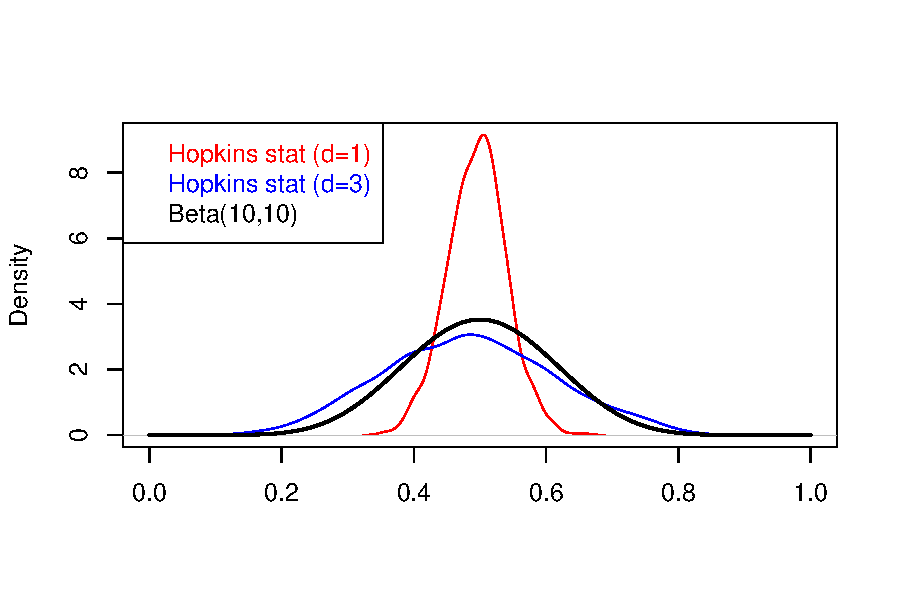
\includegraphics[width=0.9\linewidth]{RJ-2022-055_files/figure-latex/simulation-1} 

}

\caption{Results of a simulation study of the distribution of Hopkins statistic. The red and blue lines are the empirical density curves of 1000 Hopkins statistics calculated with exponents $d=1$ (red) and $d=3$ (blue). The black line is the theoretical distribution of the Hopkins statistic. The red line is very far away from the black line and shows that calculating Hopkins statistic with exponent $d=1$ is incorrect.}\label{fig:simulation}
\end{figure}

In Figure \ref{fig:simulation}:

\begin{itemize}
\tightlist
\item
  The black curve is the density of Beta(10,10).
\item
  The red curve is the density of Hopkins statistic when \(d=1\) is used in the calculation (incorrect).
\item
  The blue curve is the density of Hopkins statistic when \(d=3\) (the number of columns in \(X\)) is used (correct).
\end{itemize}

The empirical density of the blue curve is similar to the theoretical distribution shown by the black line. The empirical density of the red curve is clearly dissimilar. The distribution of Hopkins statistic with \(d=1\) is clearly incorrect (except in trivial cases where \(X\) has only 1 column). One more thing to note about the graph is that the blue curve is slightly flatter than the theoretical distribution shown in black. This is not accidental, but is caused by edge effects of the sampling region and will be discussed in a later section.

\hypertarget{examples}{%
\section{Examples}\label{examples}}

The first three examples in this section are adapted from Gastner (2005). The datasets are available in the \href{https://cran.r-project.org/web/packages/spatstat.data/index.html}{spatstat.data} package (Baddeley, Turner, and Rubak 2021). A modified version of the \texttt{hopkins()} function was written for this paper to show how the Hopkins statistic is calculated (inspired by Figure 1 of Lawson and Jurs (1990)). In order to minimize the amount of over-plotting, only \(m=3\) sampling points are used for these examples. In each figure, 3 of the existing events in \(X\) are chosen at random and a light-blue arrow is drawn to the nearest neighbor in \(X\). In addition, 3 points are drawn uniformly in the plotting region and a light-red arrow is drawn to the nearest neighbor in \(X\). The colored numbers are the lengths of the arrows.

\hypertarget{example-1-systematically-spaced-data}{%
\subsection{Example 1: Systematically-spaced data}\label{example-1-systematically-spaced-data}}

\begin{figure}

{\centering 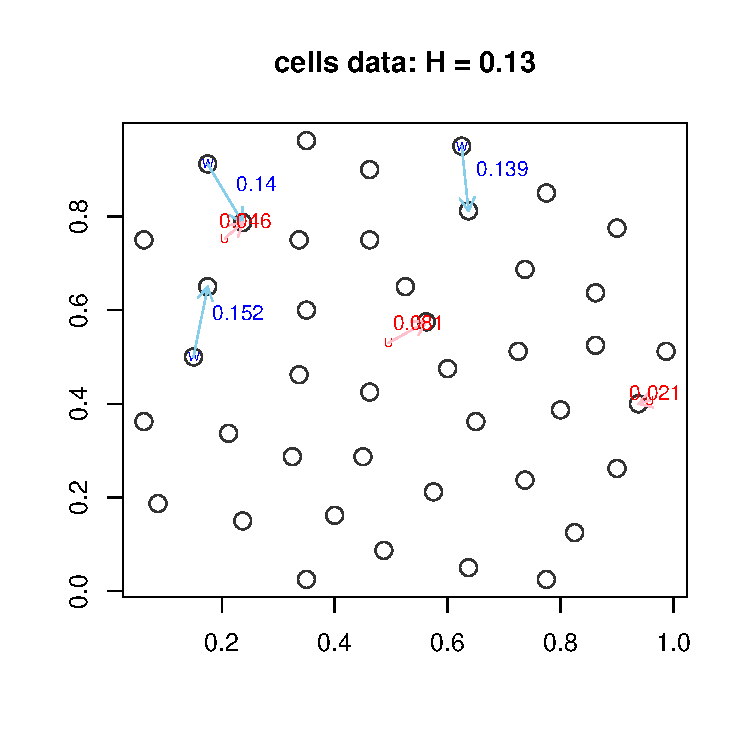
\includegraphics[width=0.6\linewidth]{RJ-2022-055_files/figure-latex/cells-1} 

}

\caption{An example of how Hopkins statistic is calculated with systematically-spaced data. The black circles are the events of the `cells` data. Each blue `W` represents a randomly-chosen event. Each blue arrow points from a `W` to the nearest-neighboring event. Each red `U` is a new, randomly-generated point. Each red arrow points from a `U` to the nearest-neighboring event. The numbers are the length of the arrows. In systematically-spaced data, red arrows tend to be shorter than blue arrows.}\label{fig:cells}
\end{figure}

The \texttt{cells} data represent the centers of mass of 42 cells from insect tissue. The scatterplot of the data in Figure \ref{fig:cells} shows that events are systematically spaced as nearly far apart as possible. Because the data is two-dimensional, Hopkins statistics is calculated as the sum of the squared distances \(u_i^2\) divided by the sum of the squared distances \(u_i^2 + w_i^2\):

\begin{verbatim}
(.046^2 + .081^2 + .021^2) / 
  ( (.046^2 + .081^2 + .021^2) + (.152^2 + .14^2 + .139^2) )
\end{verbatim}

\begin{verbatim}
#> [1] 0.1281644
\end{verbatim}

The \texttt{hopkins()} function returns the same value:

\begin{verbatim}
set.seed(17)
hopkins(cells, m=3)
\end{verbatim}

\begin{verbatim}
#> [1] 0.1285197
\end{verbatim}

The value of the Hopkins statistic in this calculation is based on only \(m=3\) events and will have sizable sampling error. To reduce the sampling error, a larger sample size can be used up to approximately 10\% of the number of events. To reduce sampling error further while maintaining the independence assumption of the sampling in calculating Hopkins statistic, repeated samples can be drawn. Here we use the idea of Gastner (2005) to calculate Hopkins statistic 100 times and then calculate the mean and standard deviation for the 100 values of Hopkins statistic, which in this case are 0.21 and 0.06. This value of the statistic is quite a bit lower than 0.5 and indicates the events are spaced more evenly than purely-random events (p-value 0.05).

\hypertarget{example-2-randomly-spaced-data}{%
\subsection{Example 2: Randomly-spaced data}\label{example-2-randomly-spaced-data}}

The \texttt{japanesepines} data contains the locations of 65 Japanese black pine saplings in a square 5.7 meters on a side. The plot of the data in Figure \ref{fig:japanesepines} is an example of data in which the events are randomly spaced.

\begin{figure}

{\centering 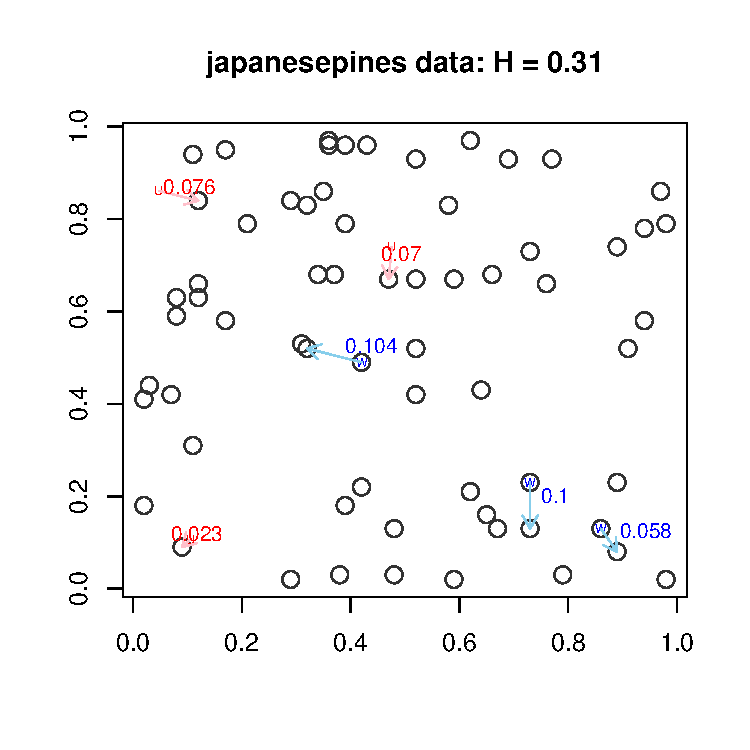
\includegraphics[width=0.6\linewidth]{RJ-2022-055_files/figure-latex/japanesepines-1} 

}

\caption{An example of how Hopkins statistic is calculated with randomly-spaced data. The black circles are the events of the `japanesepines` data. Each blue `W` represents a randomly-chosen event. Each blue arrow points from a `W` to the nearest-neighboring event. Each red `U` is a new, randomly-generated point. Each red arrow points from a `U` to the nearest-neighboring event. The numbers are the length of the arrows. In randomly-spaced data, red arrows tend to be similar in length to blue arrows.}\label{fig:japanesepines}
\end{figure}

The value of Hopkins statistic using 3 events and points is:

\begin{verbatim}
(.023^2+.076^2+.07^2) /
  ((.023^2+.076^2+.07^2) + (.104^2+.1^2+.058^2))
\end{verbatim}

\begin{verbatim}
#> [1] 0.3166596
\end{verbatim}

The mean and standard deviation of the 100 Hopkins statistics are 0.48 and 0.12. The value of the statistic is close to 0.5 and indicates no evidence against a random distribution of data (p-value 0.9).

\hypertarget{example-3-clustered-data}{%
\subsection{Example 3: Clustered data}\label{example-3-clustered-data}}

\begin{figure}

{\centering 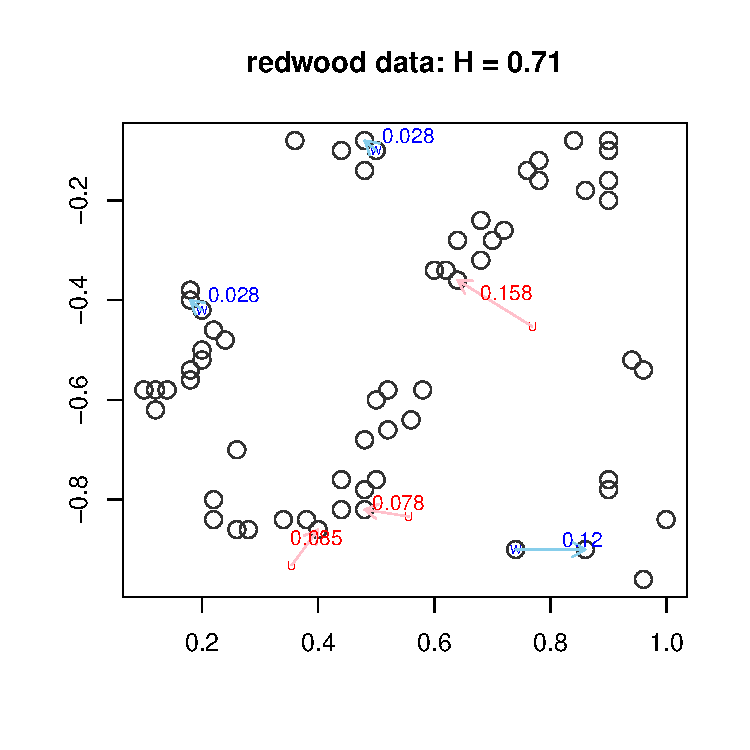
\includegraphics[width=0.6\linewidth]{RJ-2022-055_files/figure-latex/redwood-1} 

}

\caption{An example of how Hopkins statistic is calculated with clustered data. The black circles are the events of the `redwood` data. Each blue `W` represents a randomly-chosen event. Each blue arrow points from a `W` to the nearest-neighboring event. Each red `U` is a new, randomly-generated point. Each red arrow points from a `U` to the nearest-neighboring event. The numbers are the length of the arrows. In clustered data, red arrows tend to be longer in length than blue arrows.}\label{fig:redwood}
\end{figure}

The \texttt{redwood} data are the coordinates of 62 redwood seedlings in a square 23 meters on a side. The plot in Figure \ref{fig:redwood} shows events that exhibit clustering. The value of Hopkins statistic for the plot is:

\begin{verbatim}
(.085^2+.078^2+.158^2) /
  ((.085^2+.078^2+.158^2) + (.028^2+.028^2+.12^2))
\end{verbatim}

\begin{verbatim}
#> [1] 0.7056101
\end{verbatim}

The mean and standard deviation of the 100 Hopkins statistics are 0.79 and 0.13. The value of the statistic is much higher than 0.5, which indicates that the data are somewhat clustered (p-value 0.03).

\hypertarget{example-4}{%
\subsection{Example 4}\label{example-4}}

Adolfsson, Ackerman, and Brownstein (2017) provide a review of various methods of detecting clusterability. One of the methods they considered was Hopkins statistic, which they calculated using 10\% sampling. They evaluated the clusterability of nine R datasets by calculating Hopkins statistic 100 times and then reporting the proportion of time that Hopkins statistic exceeded the appropriate beta quantile. We can repeat their analysis and calculate Hopkins statistic for both \(d=1\) dimension and \(d=D\) dimensions, where \(D\) is the number of columns for each dataset.

\begin{table}

\caption{\label{tab:tabstatic}In this table, `dataset` is the R dataset name, `n` is the number of rows in the data, `D` is the number of columns in the data, `Adolfsson` is the the proportion of 100 times that Hopkins statistic was significant as appearing in the paper by Adolfsson et al. (2017), `Hopkins1` is the proportion of 100 times that Hopkins statistic was significant when calculated with the exponent $d=1$ (similar to the `clustertend` package), and `HopkinsD` is the proportion of 100 times that Hopkins statistic was significant when calculated with the exponent $d=D$. Since the `Adolfsson` and `Hopkins1` columns are similar (within samling variation), it appears that Adolfsson et al. (2017) used the `clustertend` package to calculate Hopkins statistic.}
\centering
\fontsize{7}{9}\selectfont
\begin{tabular}[t]{l|r|r|r|r|r}
\hline
dataset & n & D & Adolfsson & Hopkins1 & HopkinsD\\
\hline
faithful & 272 & 2 & 1.00 & 1.00 & 1.00\\
\hline
iris & 150 & 5 & 1.00 & 1.00 & 1.00\\
\hline
rivers & 141 & 1 & 0.92 & 0.89 & 0.90\\
\hline
swiss & 47 & 6 & 0.41 & 0.25 & 0.94\\
\hline
attitude & 30 & 7 & 0.00 & 0.00 & 0.59\\
\hline
cars & 50 & 2 & 0.19 & 0.23 & 0.68\\
\hline
trees & 31 & 3 & 0.18 & 0.22 & 0.71\\
\hline
USJudgeRatings & 43 & 12 & 0.69 & 0.53 & 1.00\\
\hline
USArrests & 50 & 4 & 0.01 & 0.00 & 0.56\\
\hline
\end{tabular}
\end{table}

In Table 1:

\begin{itemize}
\tightlist
\item
  Column 1 is the name of the R dataset.
\item
  Column 2 is the number of observations \(n\).
\item
  Column 3 is the number of dimensions \(D\).
\item
  Column 4 is the proportion of 100 times that Hopkins statistic is significant as reported by Adolfsson, Ackerman, and Brownstein (2017).
\item
  Columns 5 and 6 use the \CRANpkg{hopkins} package. Column 5 is the proportion of 100 times that Hopkins statistic with exponent \(d=1\) and column 6 is the proportion of 100 times that Hopkins statistic with exponent \(d=D\) is significant.
\end{itemize}

Since the \texttt{Adolfsson} and \texttt{Hopkins1} columns are similar (within sampling variability), it appears that Adolfsson, Ackerman, and Brownstein (2017) used Hopkins statistic with \(d=1\) as the exponent. This would be expected if they had used the \CRANpkg{clustertend} package (YiLan and RuTong 2015 version 1.4) to calculate Hopkins statistic.

For a few of the datasets, there is substantial disagreement between the last two columns. For example, the \texttt{swiss} data is significantly clusterable 41\% of the time according to Adolfsson, Ackerman, and Brownstein (2017), but 94\% of the time when using Hopkins statistic with exponent \(d=D\). A scatterplot of the \texttt{swiss} data in Figure \ref{fig:swiss} shows that the data are strongly non-random, which agrees with the 94\%.

\begin{figure}

{\centering 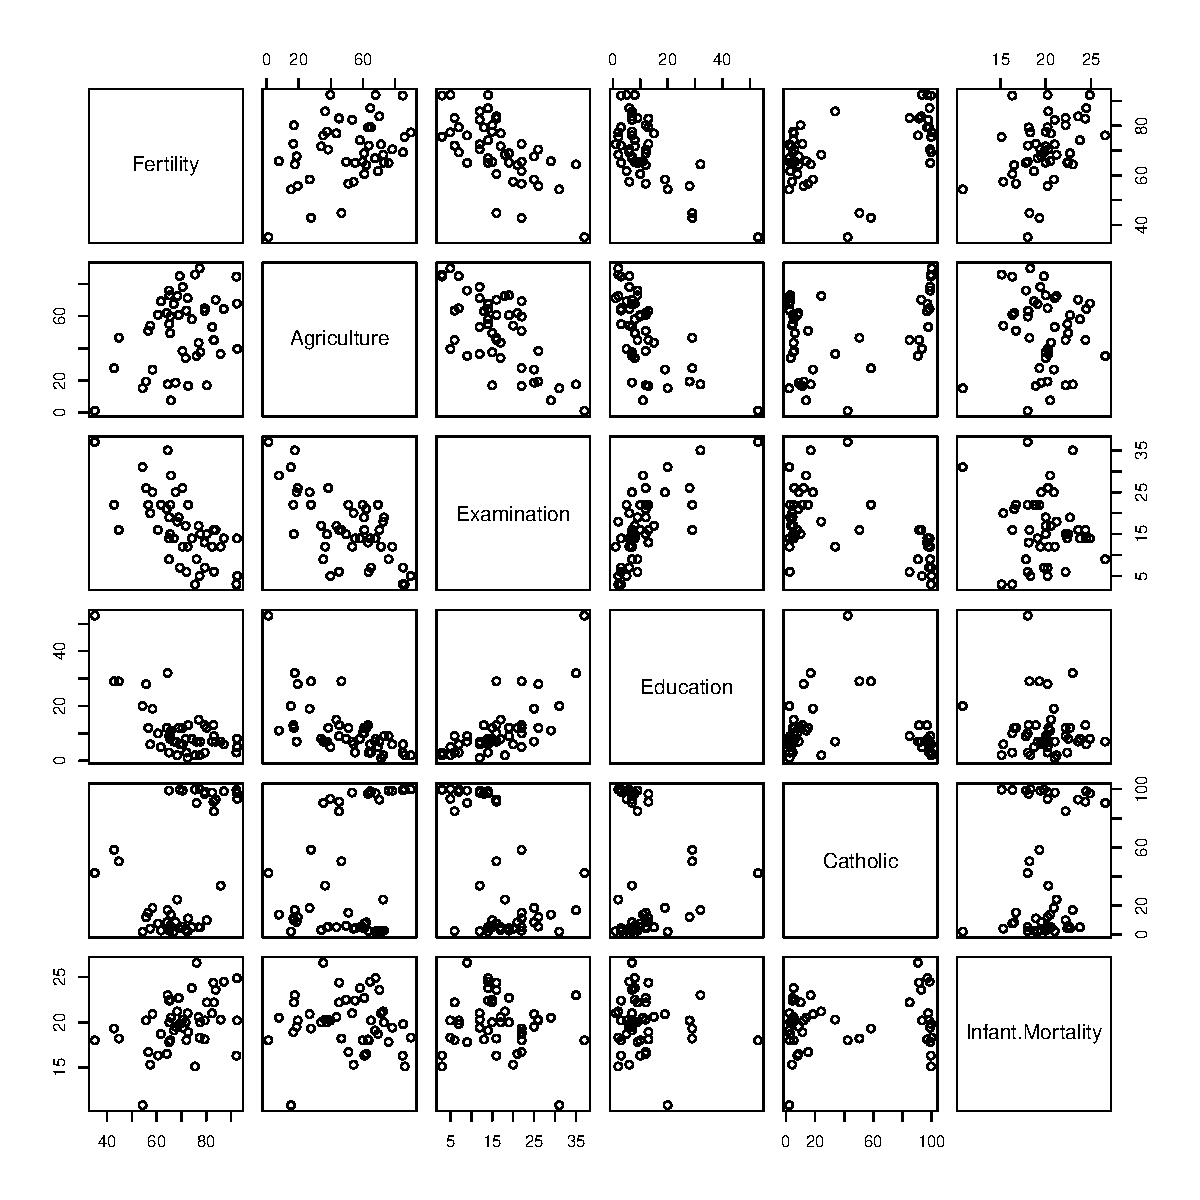
\includegraphics[width=0.9\linewidth]{RJ-2022-055_files/figure-latex/swiss-1} 

}

\caption{Pairwise scatterplots of the R dataset `swiss`. The meaning of the variables is not important here. Because some panels show a lack of spatial randomness of the data, we would expect Hopkins statistic to be significant.}\label{fig:swiss}
\end{figure}

Similarly, the \texttt{trees} data is significantly clusterable 18\% of the time according to the \texttt{Adolfsson} column, but 71\% of the time according to \texttt{HopkinsD}. The scatterplot in Figure \ref{fig:trees} shows strong non-random patterns, which agrees with the 71\%

\begin{figure}

{\centering 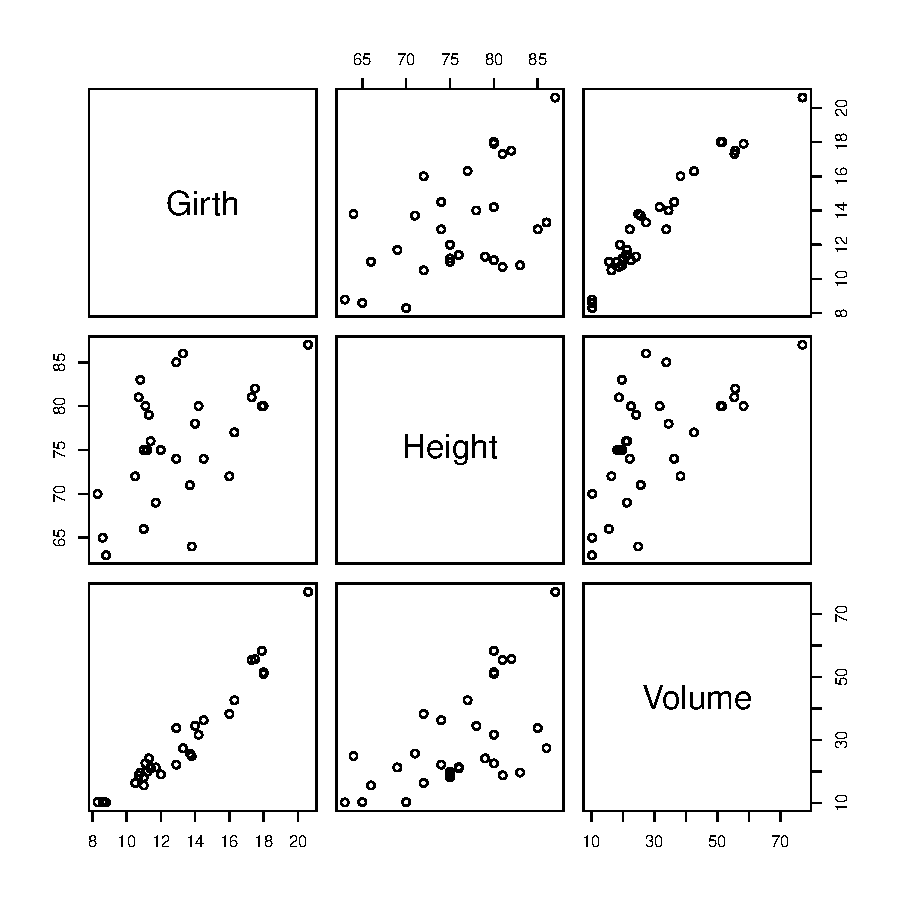
\includegraphics[width=0.7\linewidth]{RJ-2022-055_files/figure-latex/trees-1} 

}

\caption{Pairwise scatterplots of the R dataset `trees`. The data are `Girth`, `Height`, and `Volume` of 31 black cherry trees. Because all panels show a lack of spatial randomness of the data, we would expect Hopkins statistic to be significant.}\label{fig:trees}
\end{figure}

Scatterplot matrices of the \texttt{swiss}, \texttt{attitude}, \texttt{cars}, \texttt{trees}, and \texttt{USArrests} datasets can be found in Brownstein, Adolfsson, and Ackerman (2019). Each scatterplot matrix shows at least one pair of the variables with notable correlation and therefore the data are not randomly-distributed, but rather are clustered. For each of these datasets, the proportion of times \texttt{Hopkins1} is significant is less than 0.5, but the proportion of times \texttt{HopkinsD} is significant is greater than 0.5. The \texttt{HopkinsD} statistic is accurately detecting the presence of clusters in these datasets.

\hypertarget{correcting-for-edge-effects}{%
\section{Correcting for edge effects}\label{correcting-for-edge-effects}}

In the \texttt{cells}, \texttt{japanesepines} and \texttt{redwood} examples above, it is possible or even probable that there are additional events outside of the sampling frame that contains the data. The sampling frame thus has the effect of cutting off potential nearest neighbors from consideration. If the distribution of the data can be assumed to extend beyond the sampling frame and if the shape of the sampling frame can be viewed as a hypercube, then edge effects due to the sampling frame can be corrected by using a torus geometry that wraps edges of the sampling frame around to the opposite side (Li and Zhang 2007). To see an illustration of this, look again at the plot of the \texttt{japanesepines} data in Figure \ref{fig:japanesepines}. The randomly-generated event \(U\) in the upper left corner is a distance of \(0.076\) away from the nearest event. However, if the left edge of the plot is wrapped around an imaginary cylinder and connected to the right edge of the plot, then the nearest neighbor is the event in the upper-right corner at coordinates (0.97, 0.86).

To see what effect the torus geometry has on the distribution of the Hopkins statistic, consider the following simulation. We generate \(n=100\) events uniformly in a \(D=5\) dimension unit cube and sample \(m=10\) events to calculate the value of Hopkins statistic using both a simple geometry and a torus geometry. Repeat these steps \(B=1000\) times. The calculation of the nearest neighbor using a torus geometry is computationally more demanding than using a simple geometry, especially as the number of dimensions \(D\) increases, so the use of parallel computing can reduce the computing time linearly according to the number of processors used. As a point of reference, this small simulation study was performed in less than 1 minute on a reasonably-powerful laptop with 8 cores using the \CRANpkg{doParallel} package (Microsoft Corporation and Weston 2020). We found that \(B=1000\) provided results that were stable, regardless of the seed value for the random number generation in the simulations.

\begin{figure}

{\centering 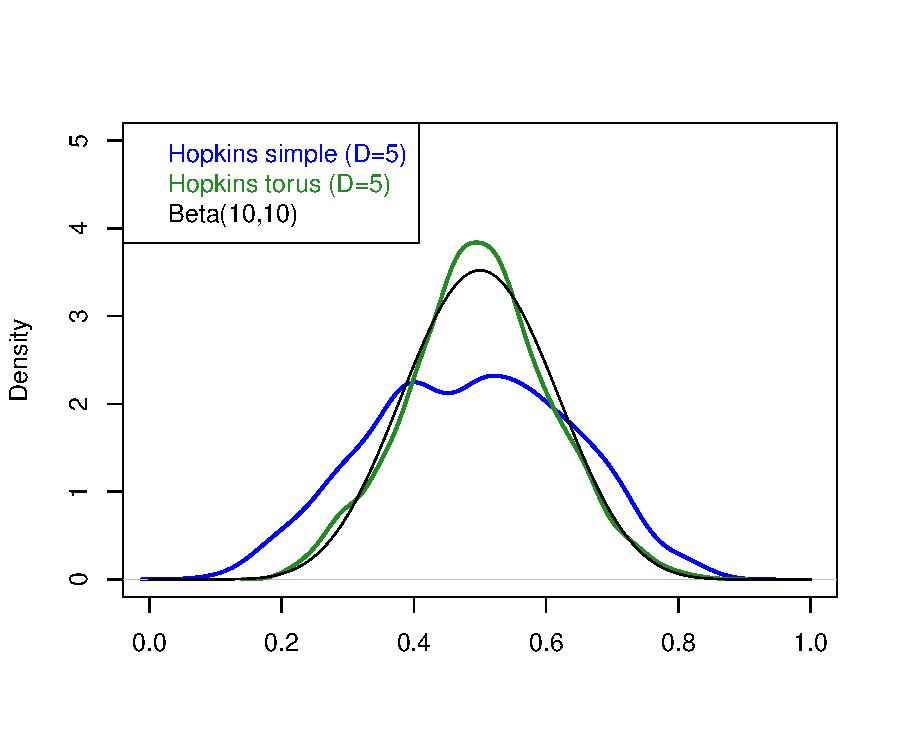
\includegraphics[width=0.9\linewidth]{RJ-2022-055_files/figure-latex/torus-1} 

}

\caption{Results of a simulation study considering how the spatial geometry affects Hopkins statistic. The thin black line is the theoretical distribution of Hopkins statistic. The blue and green lines are the empirical density curves of 1000 Hopkins statistics calculated with simple geometry (blue) and torus geometry (green). Calculating Hopkins statistic with a torus geometry aligns closely to the theoretical distribution.}\label{fig:torus}
\end{figure}

In Figure \ref{fig:torus}:

\begin{itemize}
\tightlist
\item
  The black curve is the density of Beta(10,10).
\item
  The blue curve is the empirical density of the 1000 values of Hopkins statistic calculated using a \emph{simple} geometry.
\item
  The green curve is the empirical density of the 1000 values of Hopkins statistic calculated using a \emph{torus} geometry.
\end{itemize}

When using a torus geometry to correct for edge effects in this example, the empirical distribution of Hopkins statistic is remarkably close to its theoretical distribution. In contrast, when a simple geometry is used, the empirical distribution of Hopkins statistic is somewhat flattened with heavier tails. The practical result is that when no edge correction is used, the Hopkins statistic is more likely to deviate from 0.5 and therefore more likely to suggest the data is not uniformly distributed. This erroneous interpretation is a greater risk as the number of dimensions \(D\) increases and edge effects become more pronounced

\hypertarget{sampling-frame-effects}{%
\section{Sampling frame effects}\label{sampling-frame-effects}}

\begin{figure}

{\centering 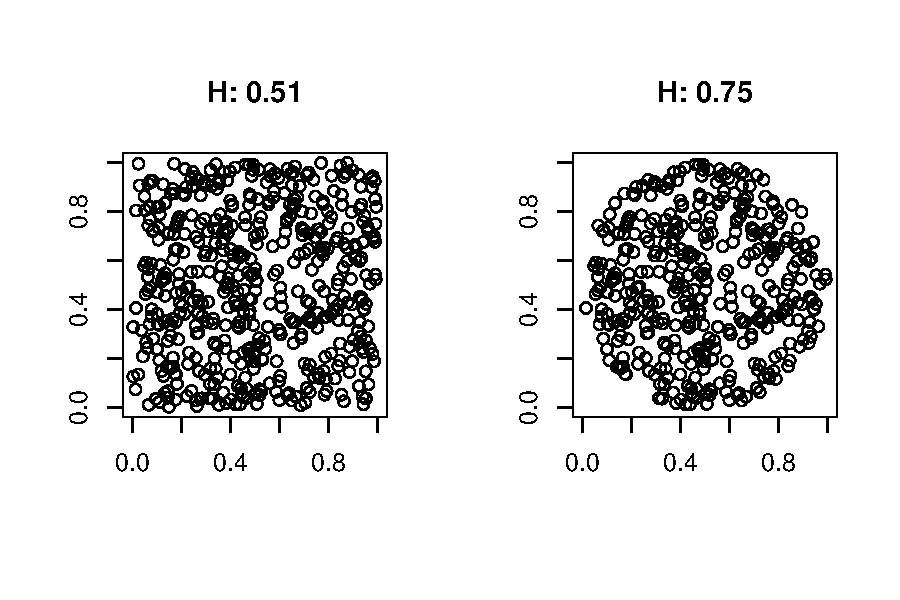
\includegraphics[width=0.9\linewidth]{RJ-2022-055_files/figure-latex/frame-1} 

}

\caption{The left figure shows 250 points simulated randomly in a unit square. As expected, the value of Hopkins statistic is close to 0.5. The right figure shows the same points, but only those inside a unit-diameter circle. The value of Hopkins statistic H is much larger than 0.5. Although both figures depict spatially-uniform points, the square shape of the sampling frame affects the value of Hopkins statistic.}\label{fig:frame}
\end{figure}

Another practical problem affecting the correct use and interpretation of Hopkins statistic has to do with the shape of the sampling frame. Consider the example data in Figure \ref{fig:frame}. On the left side, there were 250 random events simulated in a 2-dimensional unit square. On the right side, the same data are used, but have been subset to keep only the events inside a unit-diameter circle. For both figures, Hopkins statistic was calculated 100 times with 10 events sampled each time.

On the left side, both the bounding box and the actual sampling frame are the unit square. The median of 100 Hopkins statistics is 0.51, providing no evidence against random distribution. On the right side, the actual sampling frame of the data is a unit-circle, but the Hopkins statistic still uses the unit square (for generating new points in \(U\)) and the median Hopkins statistic is 0.75, indicating clustering of the data \emph{within the sampling frame}, even though the distribution of the data was generated uniformly. A few more examples of problems related to the sampling frame can be found in Smith and Jain (1984).

To consider the problem with the sampling frame on real data, refer again to the \texttt{trees} data in Figure \ref{fig:trees}. Because trees usually grow both in height and girth at the same time, it would be unexpected to find tall trees with narrow girth or short trees with large girth. Also, since the volume is a function of the girth and height, it is correlated with those two variables. In the scatterplot of girth versus volume, it would be nearly impossible to find points in the upper left or lower right corner of the square. From a biological point of view, the sampling frame cannot be shaped like a square and the null hypothesis of uniform distribution of data is violated \emph{a priori}, which means the distribution of Hopkins statistic does not follow a Beta(\(m\),\(m\)) distribution.

\hypertarget{a-protocol-for-using-hopkins-statistic}{%
\section{A protocol for using Hopkins statistic}\label{a-protocol-for-using-hopkins-statistic}}

Because Hopkins statistic is not hard to calculate and is easy to interpret, yet can be misused (as shown in the previous sections), we propose a protocol for using Hopkins statistic. The protocol simply asks the practitioner to consider the following five questions before calculating Hopkins statistic.

\begin{enumerate}
\def\labelenumi{\arabic{enumi}.}
\tightlist
\item
  \textbf{Is the number of events \(\mathbf{n > 100}\) and the number of randomly-sampled events at most 10\% of \(\mathbf{n}\)?} This is recommended by Cross and Jain (1982).
\item
  \textbf{Is spatial randomness of the events even possible?} If the events are known or suspected to be correlated, this violates the null hypothesis of spatial uniformity, and may also mean that the sampling frame is not shaped like a hypercube.
\item
  \textbf{Could nearest-neighbor events have occurred outside the boundary of the sampling frame?} If yes, it may be appropriate to calculate nearest-neighbor distances using a torus geometry.
\item
  \textbf{Is the sampling frame non-rectangular?} If yes, then be extremely careful with the use of Hopkins statistic in how points are samples from \(U\).
\item
  \textbf{Is the dimension of the data much greater than 2?} Edge effects are more common in higher dimensions.
\end{enumerate}

The important point of this protocol is to raise awareness of potential problems. We leave it to the practitioner to decide what do with the answers to these questions.

\hypertarget{conclusion}{%
\section{Conclusion}\label{conclusion}}

The statistical literature regarding Hopkins statistic is filled with confusion about how to calculate the statistic. Some publications have erroneously used the exponent \(d=1\) in the formula for Hopkins statistic and this error has propagated into much statistical software and led to incorrect conclusions. To remedy this situation, the R package \CRANpkg{hopkins} (Wright 2022) provides a function \texttt{hopkins()} that calculates Hopkins statistic using the general exponent \(d=D\) for D-dimensional data. The function can use simple geometry for fast calculations or torus geometry to correct for edge effects. Using this function, we show that the distribution of Hopkins statistic calculated with the general exponent \(d=D\) aligns closely with the theoretical distribution of the statistic. Because inference with Hopkins statistic can be trickier than expected, we introduce a protocol of five questions to consider when using Hopkins statistic.

Alternative versions of Hopkins statistic have been examined by Zeng and Dubes (1985b), Rotondi (1993), Li and Zhang (2007). Other methods of examining multivariate uniformity of data have been considered by Smith and Jain (1984), Yang and Modarres (2017), and Petrie and Willemain (2013).

\hypertarget{acknowledgements}{%
\section{Acknowledgements}\label{acknowledgements}}

Thanks to Deanne Wright for bringing the confusion about Hopkins statistic to our attention.
Thanks to Vanessa Windhausen and Deanne Wright for reading early drafts of this paper and to Dianne Cook for reviewing the final version.
Thanks to Wong (2013) for the \CRANpkg{pdist} package for fast computation of nearest neighbors and thanks to Northrop (2021) for the \CRANpkg{donut} package for nearest neighbor search on a torus.

\hypertarget{references}{%
\section*{References}\label{references}}
\addcontentsline{toc}{section}{References}

\hypertarget{refs}{}
\begin{CSLReferences}{1}{0}
\leavevmode\vadjust pre{\hypertarget{ref-adolfsson2017cluster}{}}%
Adolfsson, Andreas, Margareta Ackerman, and Naomi C Brownstein. 2017. {``To Cluster, or Not to Cluster: How to Answer the Question.''} \emph{Proceedings of Knowledge Discovery from Data, Halifax, Nova Scotia, Canada, August 13-17 (TKDD '17)}. \url{https://maya-ackerman.com/wp-content/uploads/2018/09/clusterability2017.pdf}.

\leavevmode\vadjust pre{\hypertarget{ref-baddeley2021spatstat}{}}%
Baddeley, Adrian, Rolf Turner, and Ege Rubak. 2021. \emph{{spatstat.data}: Datasets for 'Spatstat' Family}. \url{https://CRAN.R-project.org/package=spatstat.data}.

\leavevmode\vadjust pre{\hypertarget{ref-banerjee2004validating}{}}%
Banerjee, Amit, and Rajesh N Dave. 2004. {``Validating Clusters Using the {Hopkins} Statistic.''} In \emph{2004 IEEE International Conference on Fuzzy Systems (IEEE Cat. No. 04CH37542)}, 1:149--53. IEEE. \url{https://doi.org/10.1109/FUZZY.2004.1375706}.

\leavevmode\vadjust pre{\hypertarget{ref-brownstein2019descriptive}{}}%
Brownstein, Naomi C, Andreas Adolfsson, and Margareta Ackerman. 2019. {``Descriptive Statistics and Visualization of Data from the {R} Datasets Package with Implications for Clusterability.''} \emph{Data in Brief} 25: 104004. \url{https://doi.org/10.1016/j.dib.2019.104004}.

\leavevmode\vadjust pre{\hypertarget{ref-cross1982measurement}{}}%
Cross, G R, and A K Jain. 1982. {``Measurement of Clustering Tendency.''} In \emph{Theory and Application of Digital Control}, 315--20. \url{https://doi.org/10.1016/B978-0-08-027618-2.50054-1}.

\leavevmode\vadjust pre{\hypertarget{ref-diggle1976statistical}{}}%
Diggle, Peter J, Julian Besag, and J Timothy Gleaves. 1976. {``Statistical Analysis of Spatial Point Patterns by Means of Distance Methods.''} \emph{Biometrics}, 659--67. \url{https://doi.org/10.2307/2529754}.

\leavevmode\vadjust pre{\hypertarget{ref-dubes1987test}{}}%
Dubes, Richard C, and Guangzhou Zeng. 1987. {``A Test for Spatial Homogeneity in Cluster Analysis.''} \emph{Journal of Classification} 4 (1): 33--56. \url{https://doi.org/10.1007/BF01890074}.

\leavevmode\vadjust pre{\hypertarget{ref-gastner2005spatial}{}}%
Gastner, Michael T. 2005. {``Spatial Distributions: Density-Equalizing Map Projections, Facility Location, and Two-Dimensional Networks.''} PhD thesis, Univ. Michigan. \url{https://hdl.handle.net/2027.42/125368}.

\leavevmode\vadjust pre{\hypertarget{ref-hopkins1954new}{}}%
Hopkins, Brian, and John Gordon Skellam. 1954. {``A New Method for Determining the Type of Distribution of Plant Individuals.''} \emph{Annals of Botany} 18 (2): 213--27. \url{https://doi.org/10.1093/oxfordjournals.aob.a083391}.

\leavevmode\vadjust pre{\hypertarget{ref-jurs1990clustering}{}}%
Jurs, Peter C, and Richard G Lawson. 1990. {``Clustering Tendency Applied to Chemical Feature Selection.''} \emph{Drug Information Journal} 24 (4): 691--704. \url{https://doi.org/10.1177/216847909002400405}.

\leavevmode\vadjust pre{\hypertarget{ref-lawson1990new}{}}%
Lawson, Richard G, and Peter C Jurs. 1990. {``New Index for Clustering Tendency and Its Application to Chemical Problems.''} \emph{Journal of Chemical Information and Computer Sciences} 30 (1): 36--41. \url{https://doi.org/10.1021/ci00065a010}.

\leavevmode\vadjust pre{\hypertarget{ref-li2007comparison}{}}%
Li, Fasheng, and Lianjun Zhang. 2007. {``Comparison of Point Pattern Analysis Methods for Classifying the Spatial Distributions of Spruce-Fir Stands in the North-East {USA}.''} \emph{Forestry} 80 (3): 337--49. \url{https://doi.org/10.1093/forestry/cpm010}.

\leavevmode\vadjust pre{\hypertarget{ref-microsoft2020doparallel}{}}%
Microsoft Corporation, and Steve Weston. 2020. \emph{{doParallel}: Foreach Parallel Adaptor for the 'Parallel' Package}. \url{https://CRAN.R-project.org/package=doParallel}.

\leavevmode\vadjust pre{\hypertarget{ref-northrop2021donut}{}}%
Northrop, Paul J. 2021. \emph{{donut}: Nearest Neighbour Search with Variables on a Torus}. \url{https://CRAN.R-project.org/package=donut}.

\leavevmode\vadjust pre{\hypertarget{ref-petrie2013empirical}{}}%
Petrie, Adam, and Thomas R. Willemain. 2013. {``An Empirical Study of Tests for Uniformity in Multidimensional Data.''} \emph{Computational Statistics \& Data Analysis} 64: 253--68. \url{https://doi.org/10.1016/j.csda.2013.02.013}.

\leavevmode\vadjust pre{\hypertarget{ref-rotondi1993tests}{}}%
Rotondi, Renata. 1993. {``Tests of Randomness Based on the {k-NN} Distances for Data from a Bounded Region.''} \emph{Probability in the Engineering and Informational Sciences} 7: 557--69. \url{https://doi.org/10.1017/S0269964800003132}.

\leavevmode\vadjust pre{\hypertarget{ref-smith1984testing}{}}%
Smith, Stephen P, and Anil K Jain. 1984. {``Testing for Uniformity in Multidimensional Data.''} \emph{{IEEE} Transactions on Pattern Analysis and Machine Intelligence}, no. 1: 73--81. \url{https://doi.org/10.1109/TPAMI.1984.4767477}.

\leavevmode\vadjust pre{\hypertarget{ref-wong2013pdist}{}}%
Wong, Jeffrey. 2013. \emph{{pdist}: Partitioned Distance Function}. \url{https://CRAN.R-project.org/package=pdist}.

\leavevmode\vadjust pre{\hypertarget{ref-wright2022hopkins}{}}%
Wright, Kevin. 2022. \emph{{hopkins}: Calculate Hopkins Statistic for Clustering}. \url{https://CRAN.R-project.org/package=hopkins}.

\leavevmode\vadjust pre{\hypertarget{ref-yang2017multivariate}{}}%
Yang, Mengta, and Reza Modarres. 2017. {``Multivariate Tests of Uniformity.''} \emph{Statistical Papers} 58: 627--39. \url{https://doi.org/10.1007/s00362-015-0715-x}.

\leavevmode\vadjust pre{\hypertarget{ref-yilan2015clustertend}{}}%
YiLan, Luo, and Zeng RuTong. 2015. \emph{{clustertend}: Check the Clustering Tendency}. \url{https://CRAN.R-project.org/package=clustertend}.

\leavevmode\vadjust pre{\hypertarget{ref-zeng1985comparison}{}}%
Zeng, Guangzhou, and Richard C Dubes. 1985a. {``A Comparison of Tests for Randomness.''} \emph{Pattern Recognition} 18 (2): 191--98. \url{https://doi.org/10.1016/0031-3203(85)90043-3}.

\leavevmode\vadjust pre{\hypertarget{ref-zeng1985test}{}}%
---------. 1985b. {``A Test for Spatial Randomness Based on {k-NN} Distances.''} \emph{Pattern Recognition Letters} 3 (2): 85--91. \url{https://doi.org/10.1016/0167-8655(85)90013-3}.

\end{CSLReferences}

\bibliography{hopkins.bib}

\address{%
Kevin Wright\\
Corteva Agriscience\\%
6805 NW 62nd Ave\\ Johnston, IA 50131\\
%
%
\textit{ORCiD: \href{https://orcid.org/0000-0002-0617-8673}{0000-0002-0617-8673}}\\%
\href{mailto:kw.stat@gmail.com}{\nolinkurl{kw.stat@gmail.com}}%
}
